\chapter{Cenni teorici}

In questo capitolo, verrà fornita un'introduzione approfondita agli standard e alle tecnologie che sono stati considerati nell'ambito della nostra attività. La comprensione di tali standard è fondamentale per contestualizzare le scelte progettuali e le strategie implementate. Ci concentreremo su diversi protocolli e specifiche tecniche che hanno influenzato lo sviluppo delle soluzioni adottate, esplorando le loro caratteristiche distintive, le modalità di funzionamento e le applicazioni pratiche.

In particolare, analizzeremo gli standard relativi alla comunicazione wireless nell'ambito \textit{automotive}, come WAVE (\textit{Wireless Access in Vehicular Environments}), che gioca un ruolo cruciale nella connettività dei veicoli e nella gestione delle reti di trasporto intelligenti. 

Successivamente, esamineremo il meccanismo EDCA (\textit{Enhanced Distributed Channel Access}), che è una parte integrante del livello MAC (\textit{Media Access Control}) nel contesto delle reti wireless. EDCA introduce un metodo di accesso al canale più sofisticato rispetto al tradizionale DCF (\textit{Distributed Coordination Function}), permettendo una gestione più efficiente delle priorità di traffico. Questo è particolarmente importante in scenari in cui coesistono diversi tipi di traffico, come video, voce e dati, ognuno con requisiti di latenza e larghezza di banda diversi. Discuteremo come EDCA assegna diverse code di accesso per garantire che le comunicazioni più critiche ricevano la priorità necessaria, migliorando così l'esperienza complessiva degli utenti.

Attraverso questa analisi di WAVE e EDCA, il capitolo intende fornire una comprensione approfondita delle tecnologie che supportano le comunicazioni nei veicoli connessi, evidenziando come queste innovazioni possano contribuire a una mobilità più sicura ed efficiente.

\section{ITS - Intelligent Transport System}
Non so se metterli qui.

\section{VANET}
Idem come ITS.

\section{IEEE 802.11p (WAVE)}
WAVE è progettato specificamente per ambienti di trasporto, consentendo la comunicazione tra veicoli (V2V) e tra veicoli e infrastrutture stradali (V2I). Questo protocollo sfrutta canali wireless dedicati per garantire una bassa latenza e una maggiore affidabilità, elementi essenziali per applicazioni critiche come la prevenzione degli incidenti e la gestione del traffico. 

Per facilitare questo, l'IEEE ha introdotto un emendamento specifico al protocollo 802.11, noto come 802.11p\cite{std2007wireless}. Questo emendamento si occupa sia del livello fisico, chiamato PHY, sia della gestione dell'accesso al canale, che riguarda il livello MAC. Non ci soffermeremo ulteriormente sui livelli superiori, se non attraverso un breve excursus, poiché il protocollo in questione supporta senza difficoltà qualsiasi tipo di livello, sia esso basato su IP o meno\cite{DSRC-Based-vehicular}. Degno di nota è il fatto che è stato previsto un apposito protocollo per l'invio di frame che non richiedono un livello di trasporto come TCP o UDP, denominato \textit{WAVE Short Message Protocol (WSMP)}.

\begin{figure}[h!]
    \centering
    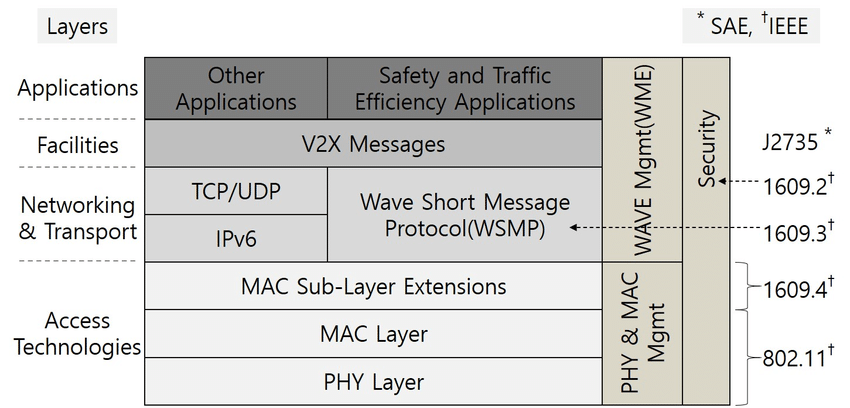
\includegraphics[width=0.7\textwidth]{WAVE-protocol-stack.png}
    \caption{Stack protocollo WAVE}
    \label{fig:etichetta}
\end{figure}

\subsection[Physical layer]{Physical layer}

\subsection[MAC layer]{MAC layer}

\subsection[EDCA]{EDCA}

\subsection[IEEE 1609.4 for multi-channel operations]{IEEE 1609.4 for multi-channel operations}